\chapter{Introduzione}
\section{Che cos'è il Brute Force}
Nella crittografia , un attacco di Brute Force consiste in un utente malintenzionato che invia molte password con la speranza di indovinare una combinazione correttamente.

L'aggressore controlla sistematicamente tutte le possibili password finché non trova quella corretta. In alternativa, l'attaccante può tentare di indovinare la chiave che in genere viene creata dalla password utilizzando una funzione di derivazione della chiave.
\begin{figure}[h]
    \centering
    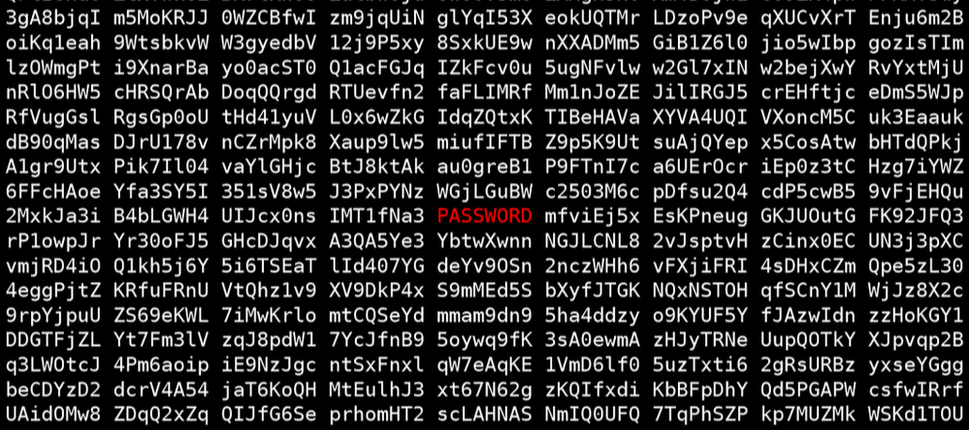
\includegraphics[width=115mm]{Immagini/introduzione/banner.png}
\end{figure}

Un attacco di Brute Force è un attacco crittoanalitico che, in teoria, può essere utilizzato per tentare di decrittografare qualsiasi dato crittografato. Tale attacco potrebbe essere utilizzato quando non è possibile sfruttare altri punti deboli in un sistema di crittografia che renderebbero il compito più semplice.

Gli attacchi di forza bruta funzionano calcolando ogni possibile combinazione che potrebbe costituire una password e testandola per vedere se è la password corretta. All'aumentare della lunghezza della password, la quantità di tempo e la potenza di calcolo richiesta in media per trovare la password corretta aumenta in modo esponenziale.

Per password più lunghe vengono utilizzati altri metodi come l' attacco del dizionario perché una ricerca a forza bruta richiede troppo tempo. Password e chiavi più lunghe hanno più valori possibili e persino più combinazioni, il che le rende esponenzialmente più difficili da decifrare rispetto a quelle più corte.

Gli attacchi di forza bruta possono essere resi meno efficaci offuscando i dati da codificare, rendendo più difficile per un utente malintenzionato riconoscere quando il codice è stato craccato o costringendo l'aggressore a fare più lavoro per testare ogni ipotesi. Una delle misure della forza di un sistema di crittografia è il tempo che teoricamente impiegherebbe un utente malintenzionato per sferrare un attacco di forza bruta riuscito contro di esso.
\section{Hash}
Le funzioni hash \cite{hash} sono particolari funzioni che permettono di dare a un messaggio un’impronta digitale tale da identificarlo univocamente.
\begin{figure}[h]
    \centering
    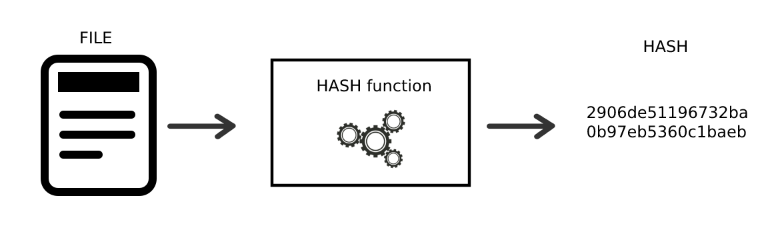
\includegraphics[width=115mm]{Immagini/introduzione/hash.png}
    \caption{hash}
    \label{fig:hash}
\end{figure}

In altre parole creano una stringa associata al messaggio da spedire e per il quale, una volta applicata la funzione, non dovrebbe essere più possibile ritornare al testo originale.
Quindi, il valore hash h(M) è una rappresentazione non ambigua e non falsificabile di un messaggio M, facile da calcolare e tale da comprimere il messaggio stesso.
Tra le principali proprietà delle funzioni hash ricordiamo che: sono facili da calcolare, godono della proprietà di sicurezza forte (è computazionalmente difficile trovare 2 messaggi diversi con lo stesso valore hash), godono della proprietà di sicurezza debole (dato M, è computazionalmente difficile trovare M’ tale che h(M) = h(M’)), e sono One-way, cioè, dato y è computazionalmente difficile trovare M tale che y = h(M).
\subsection{Types}
Le principali funzioni hash presenti attualmente sono:
\begin{itemize}
    \item \textbf{MD2}\newline  acronimo di Message Digest Algorithm, produce un valore hash di 128 bit e richiede come input multipli di 16 byte. La funzione, inoltre, usa un padding, cioè aggiunge dei bit mancanti ai messaggi in input che non hanno la lunghezza giusta. Questo algoritmo è già stato violato.
    \item \textbf{MD4}\newline anche questa funzione usa hash a 128 bit, ma è più veloce di MD2. Processa il messaggio dividendolo in blocchi di 512 bit. Il padding del messaggio, inoltre, comprende un valore di 64 bit che indica la lunghezza del messaggio originale. Questa funzione è più sicura della precedente, in quanto la difficoltà di produrre due messaggi che hanno la stessa lunghezza con modulo \(2^{64}\) è maggiore.
    \item \textbf{MD5}\newline è stato ideato dopo la violazione di MD4, su cui è basato. Il testo è diviso in blocchi 512 bit e viene generato un hash di 128 bit. E’ basato su XOR e operazioni logiche. L’unico svantaggio è dovuto dal fatto che è un po’ più lento di MD4.
    \item \textbf{SHA-1}\newline  acronimo di Secure Hash Algorithm-1 (anche SHS, Secure Hash Standard), sviluppato dal NSA su richiesta del NIST (National Institute of Standard and Technology). Utilizza gli stessi principi di MD4 e MD5. Il progetto originale del 1994 aveva il nome di SHA, poi modificato nel codice dal NSA. Produce output di 160 bit a partire da una lunghezza arbitraria. Attualmente è uno dei più sicuri, usato anche dai servizi PGP e GPG per firmare documenti.
    \item \textbf{SHA-2}\newline versione successiva a SHA-1, genera impronte di documenti da 256, 384 e 512 bit.
\end{itemize}
\section{Password analysis}
Una cosa da conoscere per effettuare un buon attacco di Brute Force, è la composizione di una password e la sua tassonomia \cite{hashcrack}, da uno studio generale delle password è stato notato che :
\begin{itemize}
    \item la lunghezza media di una password è di 7 - 9 caratteri
    \item si ha il 50\% di possibilità che una password contenga una o più vocali
    \item le donne preferiscono utilizzare nomi per le loro password e gli uomini preferiscono gli hobby
    \item i simboli più utilizzati sono : \textasciitilde, !, @, \#, \$, \%, \&, *, e ?
    \item se si utilizza un numero è il 1 o il 2 e sono utilizzati alla fine
    \item se si utilizza più di un numero, sono sequenze o numeri personali
    \item se si utilizza una lettere maiuscola, questa si trova all'inizio
    \item 66\% delle persone utilizza 1-3 password per tutti i suoi account
    \item una persona su nove ha una password basata sulle 500 password più utilizzate
    \item i paesi occidentali preferiscono le password in minuscolo e i paesi dell'est preferiscono le cifre
\end{itemize}

Le password possono contenere molte informazioni al riguardo al suo creatore, molte volte la stessa persona utilizza un pattern specifico per la creazione delle proprie password, dove andrà a cambiare piccoli dettagli tra una password e l'altra.
Questi pattern si possono suddividere in :
\begin{itemize}
    \item \textbf{Basic Pattern}\newline
          Visibile facilmente, composto da gruppi ben distinti\newline
          \begin{figure}[h]
              \centering
              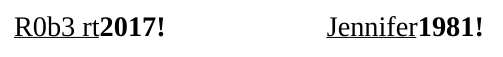
\includegraphics[width=\linewidth]{Immagini/introduzione/Basic_Pattern.png}
              \caption{Basic Pattern}
              \label{fig:basic}
          \end{figure}
          \newline Qui possiamo notare che ogni password è composta da un nome e termina con quattro numeri con lo stesso carattere speciale \!.
    \item \textbf{Macro Pattern}\newline
          Statiche sulla struttura come lunghezza e set di caratteri\newline
          \begin{figure}[h]
              \centering
              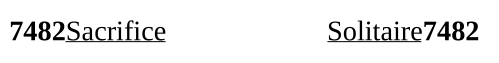
\includegraphics[width=\linewidth]{Immagini/introduzione/Macro_pattern.png}
              \caption{Macro Pattern}
              \label{fig:macro}
          \end{figure}
          \newline Qui possiamo notare che le password hanno un loro schema, composto dalla combinazione di 4 numeri e 7 lettere, inoltre la parola inizia in entrambi i casi con una maiuscola ed in entrambi i casi abbiamo sempre la stessa lettere e lo stesso gruppo di numeri.
    \item \textbf{Micro Pattern}\newline
          Utilizzo di temi e dati/interesse personali per la loro composizione\newline
          \begin{figure}[h]
              \centering
              \includegraphics[width=\linewidth]{Immagini/introduzione/Micro_Pattern.png}
              \caption{Micro Pattern}
              \label{fig:micro}
          \end{figure}
          \newline Qui possiamo notare che ogni password inizia con un colore, inoltre la seconda parte è composta da un nome di un animale e si utilizzano 3 numeri diversi per concludere la password.
\end{itemize}

L'individuazione di queste schemi possono andare a ridurre di molto i tempi che si impiegano per trovare le password, perché ci permettono di capire quale tecnica è più adeguata da applicare e quali regole applicare per l’esecuzione dell’attacco.

\subsection{20-60-20 RULE}

La regola 20-60-20 è un modo per visualizzare il livello di distribuzione delle password in base alla loro complessità, con caratteristiche che generalmente seguono quelle di una curva gaussiana, dove sull'asse delle X abbiamo la complessità della password e sul lato delle Y abbiamo il "numero" di quante persone la utilizzano.
\begin{itemize}
    \item Il 20\% delle password sono parole del dizionario facilmente indovinabili o password comuni.
    \item Il 60\% delle password sono variazioni da moderate a leggere rispetto al precedente 20\%.
    \item Il 20\% delle password sono rigide, lunghe, complesse o con caratteristiche uniche.
\end{itemize}

\begin{figure}[htpb!]
    \centering
    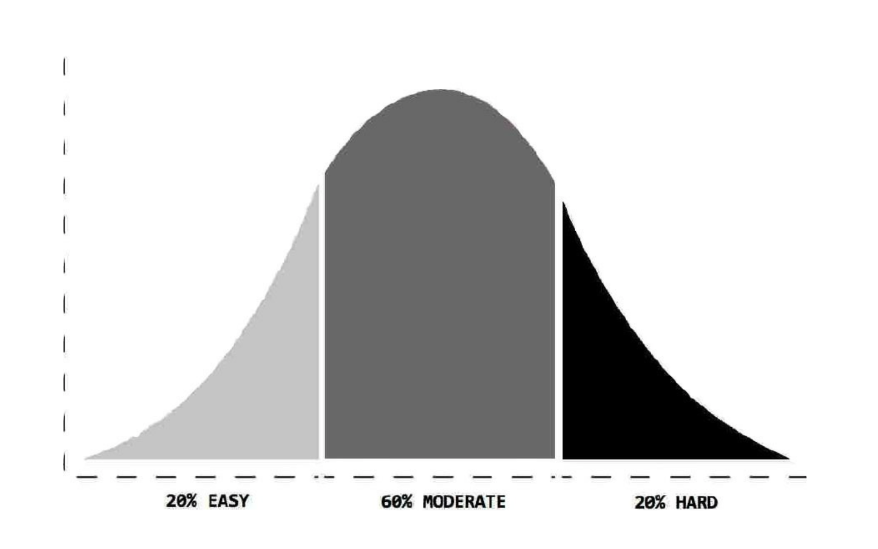
\includegraphics[width=\linewidth]{Immagini/introduzione/20-60-20.png}
    \caption{Rule 20-60-20 \cite{hashcrack}}
    \label{fig:rocker}
\end{figure}


